\chapter{SISTAL}

En este capítulo se presenta un análisis detallado del sistema actual de gestión de uniformes corporativos, SISTAL, con el propósito de comprender su funcionamiento, estructura y alcance dentro de la organización. Se describen los principales procesos operativos, sus fortalezas, oportunidades, debilidades y amenazas mediante un análisis FODA, así como la propuesta de solución orientada a su reestructuración.
Asimismo, se incluye el diseño técnico del sistema vigente, representado a través de diagramas, los cuales permiten identificar los componentes críticos y las áreas susceptibles de mejora que fundamentan la propuesta de modernización del sistema.En este capítulo se profundizará sobre el sistema actual SISTAL, los problemas que enfrenta

\section{Análisis del Problema}

En esta sección se analizan las principales problemáticas del sistema Sistal (2008), tanto técnicas como funcionales. Se caracterizan las deficiencias que afectan la eficiencia, la escalabilidad y el mantenimiento, y se establecen los fundamentos para una mejora tecnológica.


\subsection{Situación Actual}

SISTAL es una aplicación web monolítica desarrollada en PHP (2008), con base de datos MySQL sin relaciones, alojada en hosting compartido (BlueHosting) y sin control de versiones. Atiende tres actores: Administrador (empresa contratante), Funcionario (empleado) y Proveedor (confección/entrega).
Funcionalmente permite: administración de funcionarios y segmentos, captura de tallas, consolidación y envío de órdenes de confección al proveedor, seguimiento básico de estados (ingresado, confección, despacho y entrega), registro de entregas e incidencias y listados/reportes simples.

\subsubsection{Hallazgos técnicos y operativos}


\begin{itemize}
    \item \textbf{Arquitectura y datos}: monolito acoplado; modelo de datos sin normalización, lo que limita integridad y reporting.
    \item \textbf{Procesos de desarrollo}: sin control de versiones ni despliegue automatizado, sin trazabilidad de cambios ni ambientes reproducibles.
    \item \textbf{Infraestructura}: hosting compartido con latencias e inestabilidad; sin observabilidad ni alta disponibilidad.
    \item \textbf{Seguridad}: controles de acceso y cifrado insuficientes, sin prácticas DevSecOps.
    \item \textbf{UX/UI}: interfaz obsoleta y no responsive; fricción en la captura de información.
    \item \textbf{Escalabilidad}: inexistencia de multi-tenant; dificultades para servir a múltiples empresas y para integrar proveedores/logística/ERP.
\end{itemize}

\subsection{Análisis FODA}

\subsection{Solución Propuesta}

\section{Diseño del Sistema Actual}

En esta sección se documenta el diseño técnico del sistema actual, representando su estructura interna y sus principales componentes. A través de diagramas de casos de uso, base de datos, flujo, arquitectura y despliegue, se busca comprender la organización del sistema existente y las áreas que requieren modernización.


\subsection{Diagrama de Casos de Uso}

\textit{Falta ordenar el diagrama de casos de uso, por el momento se encuentra en el siguiente enlace:} \url{https://excalidraw.com/#room=80d12a9b923fafaeae02,PoQkDRXp5qahft2VZWr_gw}

\subsection{Diagrama de Bases de Datos}

Los diagramas de base de datos presentados en las Figuras \ref{fig:diagrama-bdd-1-actual} y \ref{fig:diagrama-bdd-2-actual}, son las tablas que se encuentran actualmente en el sistema. Como se aprecia, no contienen relaciones y muchas de las columnas no se utilizan.

\begin{figure}[htbp]
    \centering
    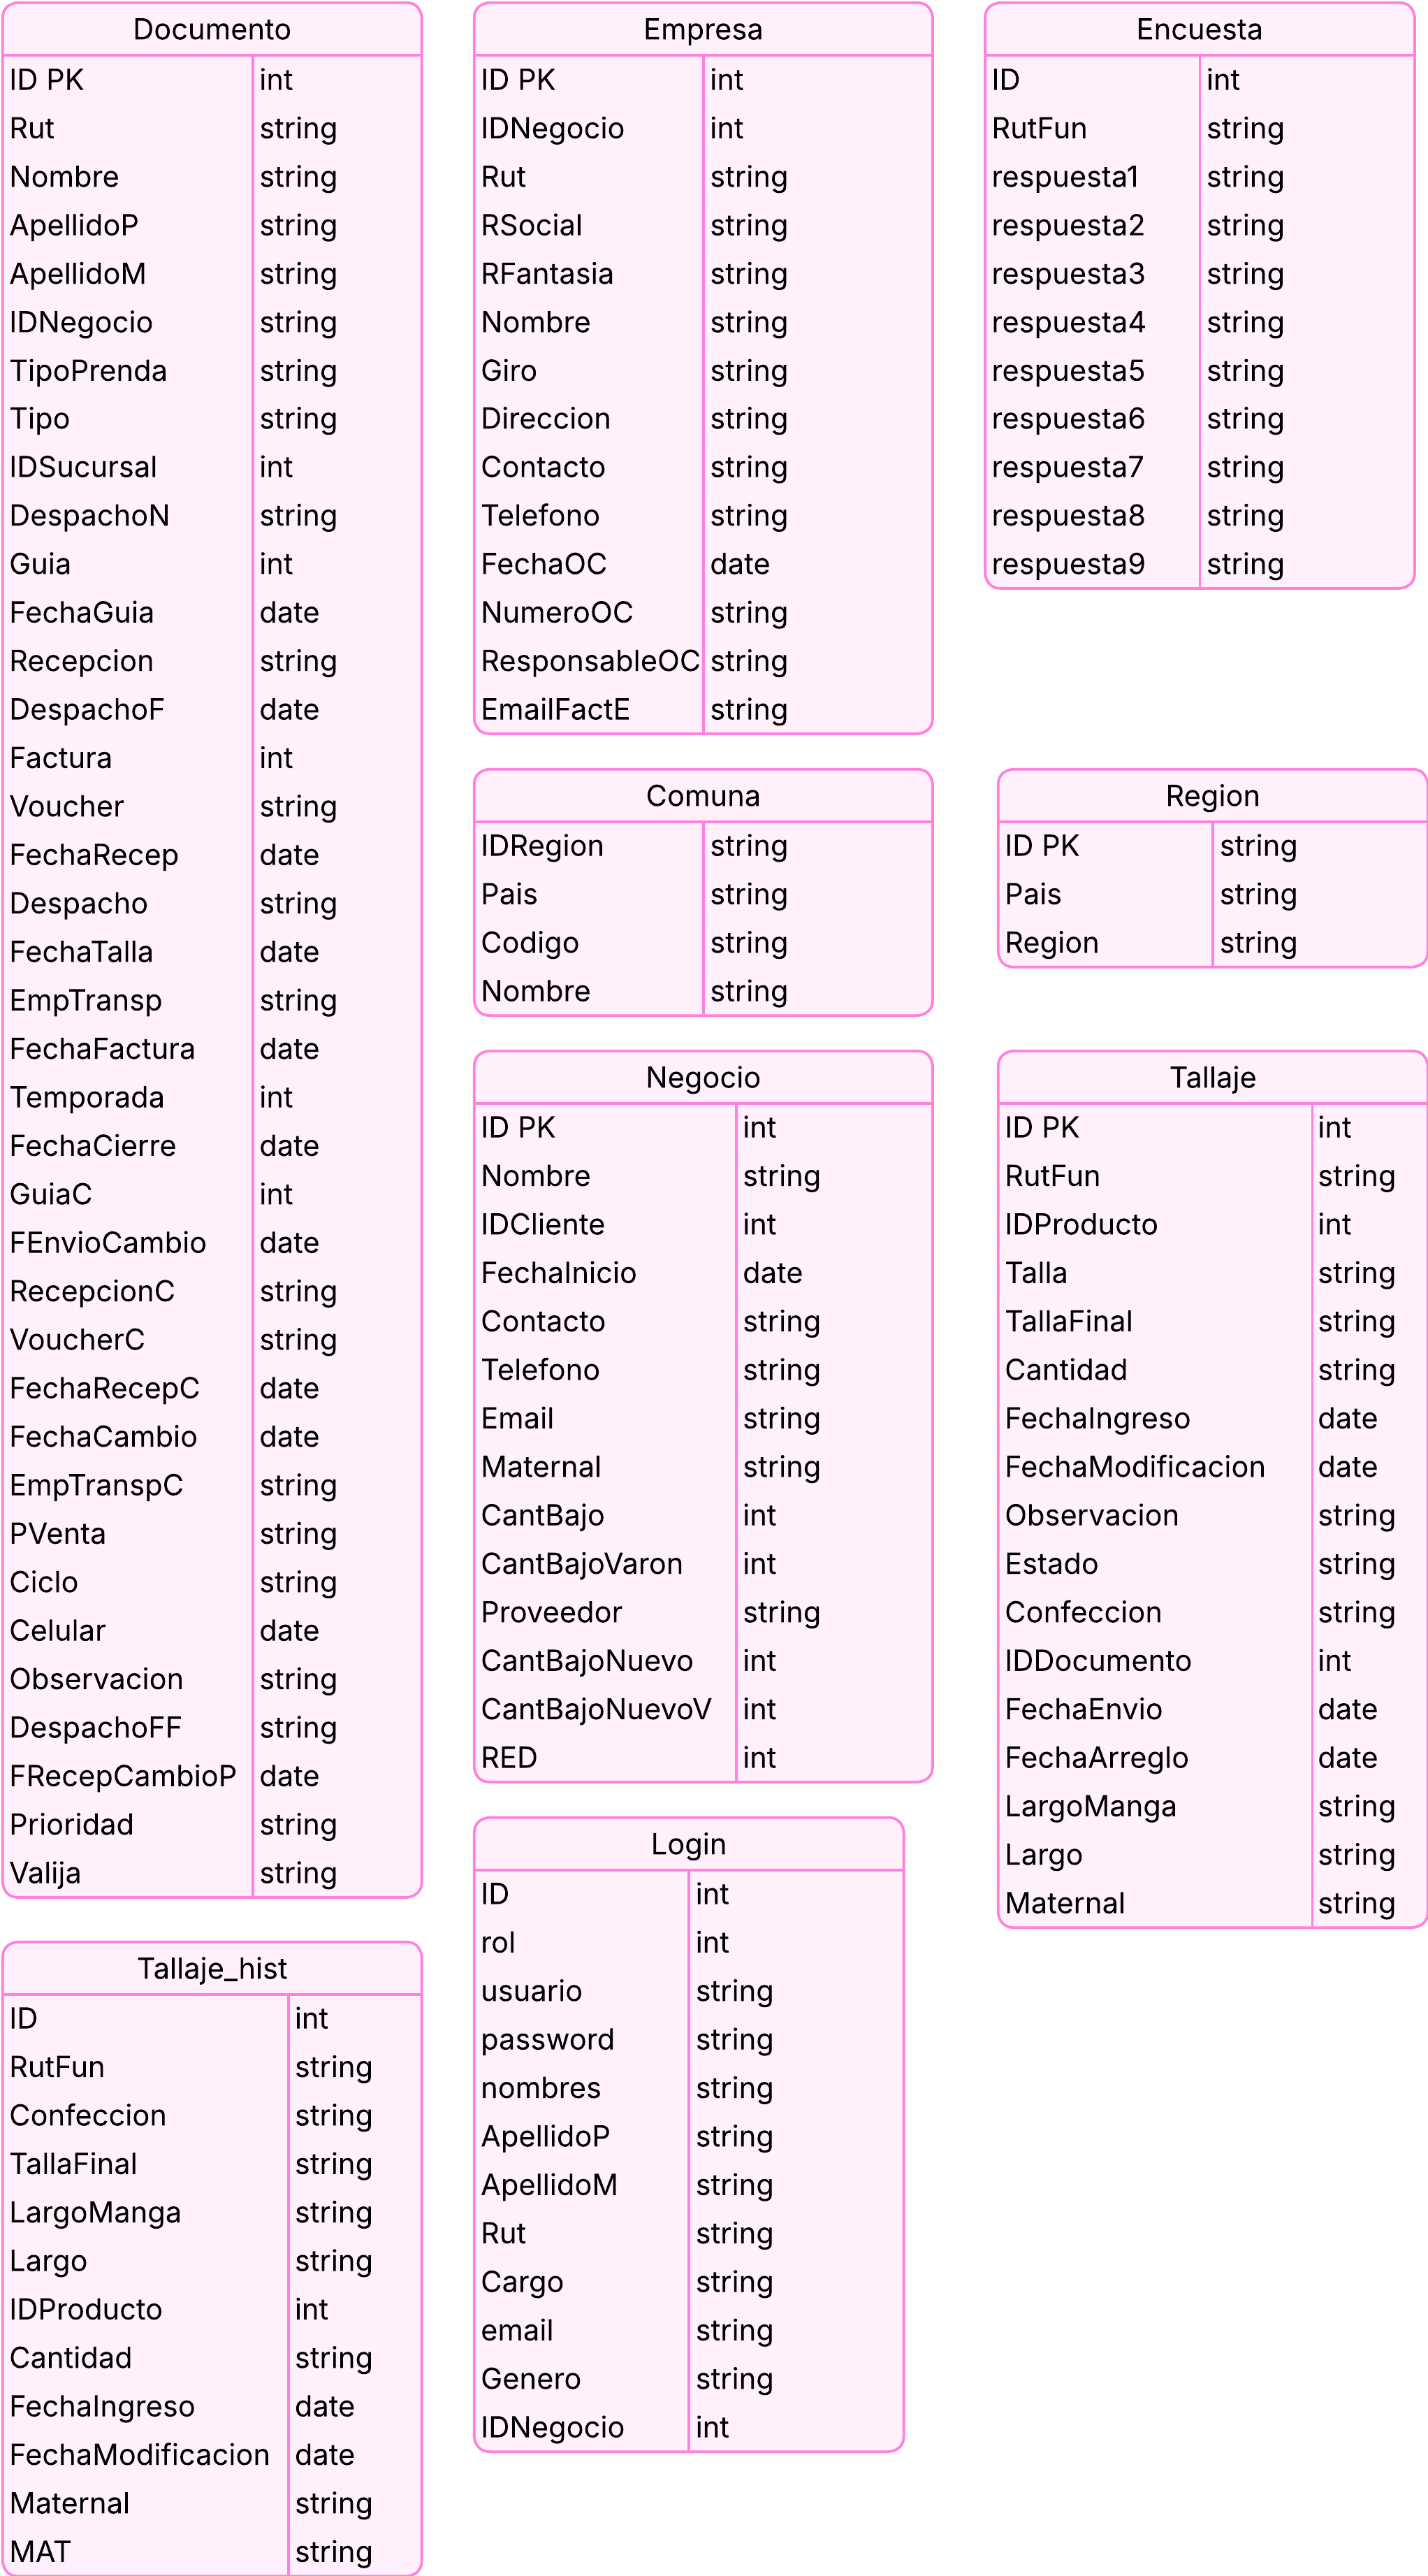
\includegraphics[height=0.9\textheight]{figuras/diagramas-actuales/diagrama-bdd-1}
    \caption{Diagrama físico de bases de datos del sistema actual (Parte 1)}
    \label{fig:diagrama-bdd-1-actual}
\end{figure}

\begin{figure}[htbp]
    \centering
    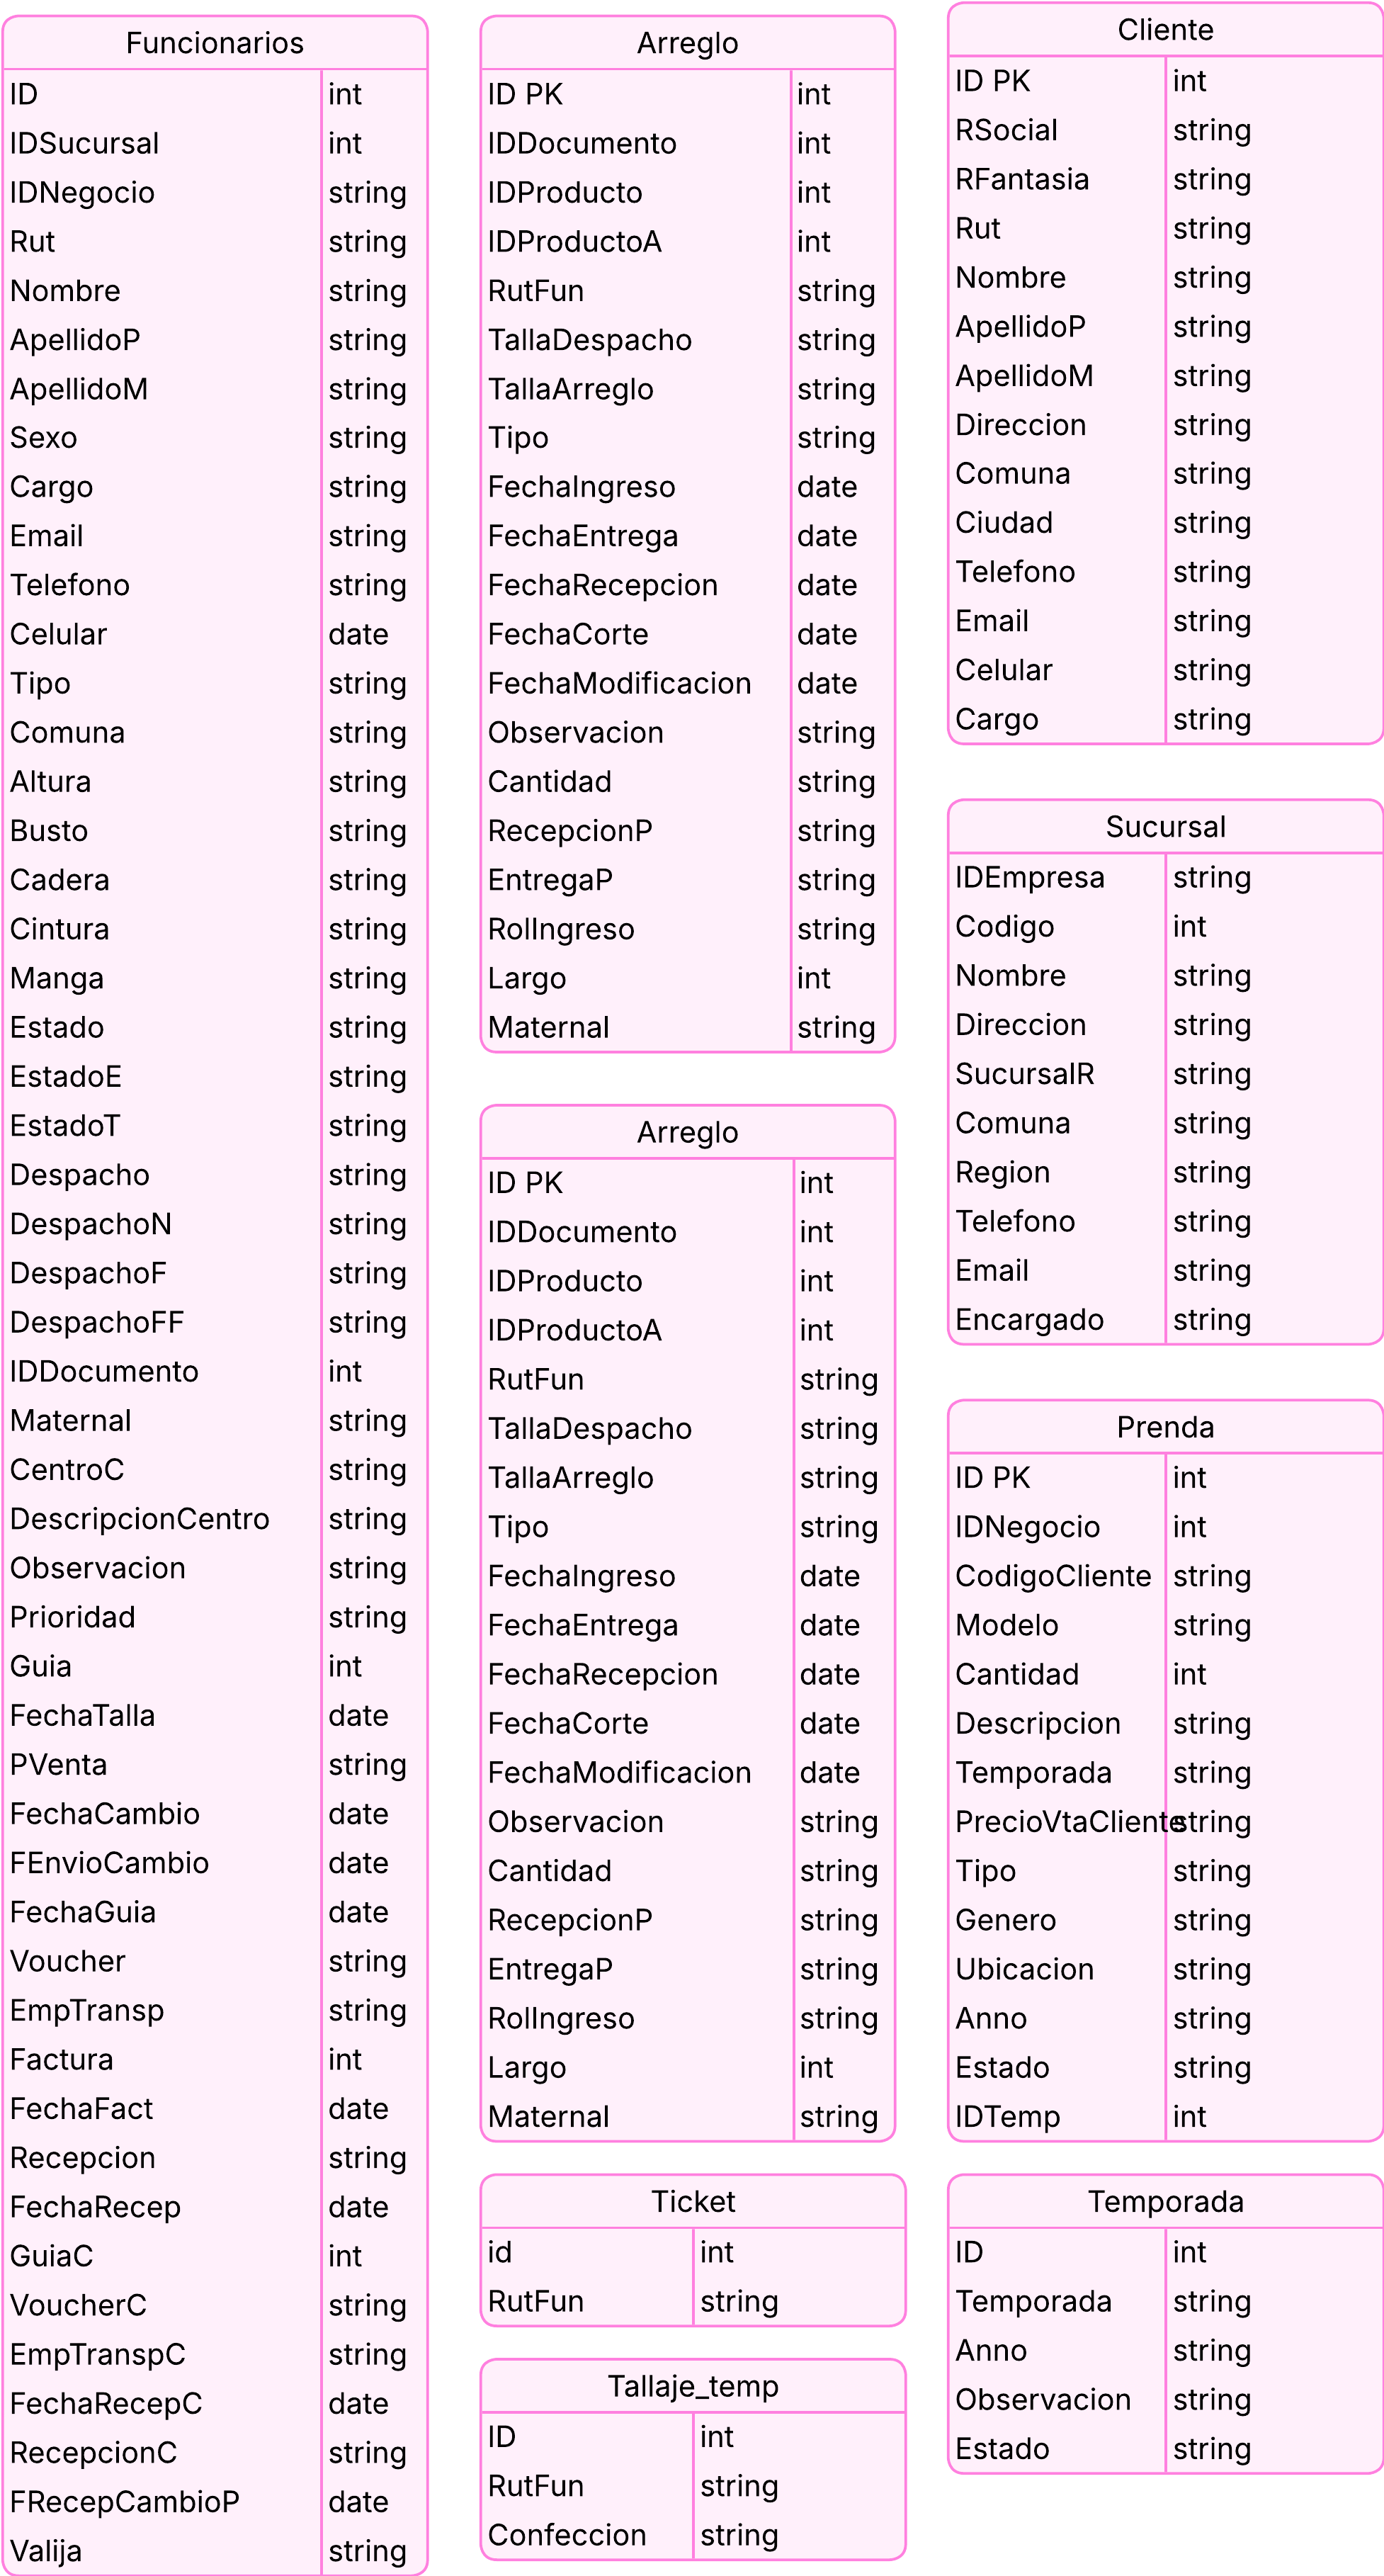
\includegraphics[height=0.9\textheight]{figuras/diagramas-actuales/diagrama-bdd-2}
    \caption{Diagrama físico de bases de datos del sistema actual (Parte 2)}
    \label{fig:diagrama-bdd-2-actual}
\end{figure}


\subsection{Diagrama de Flujo}

\textit{Falta añadir descripciones para los 3 diagramas de Flujo:} Figuras \ref{fig:diagrama-flujo-actual-registro-de-tallas}, \ref{fig:diagrama-flujo-actual-envio-a-confeccion} y \ref{fig:diagrama-flujo-actual-post-venta}.

\begin{figure}[htbp]
    \centering
    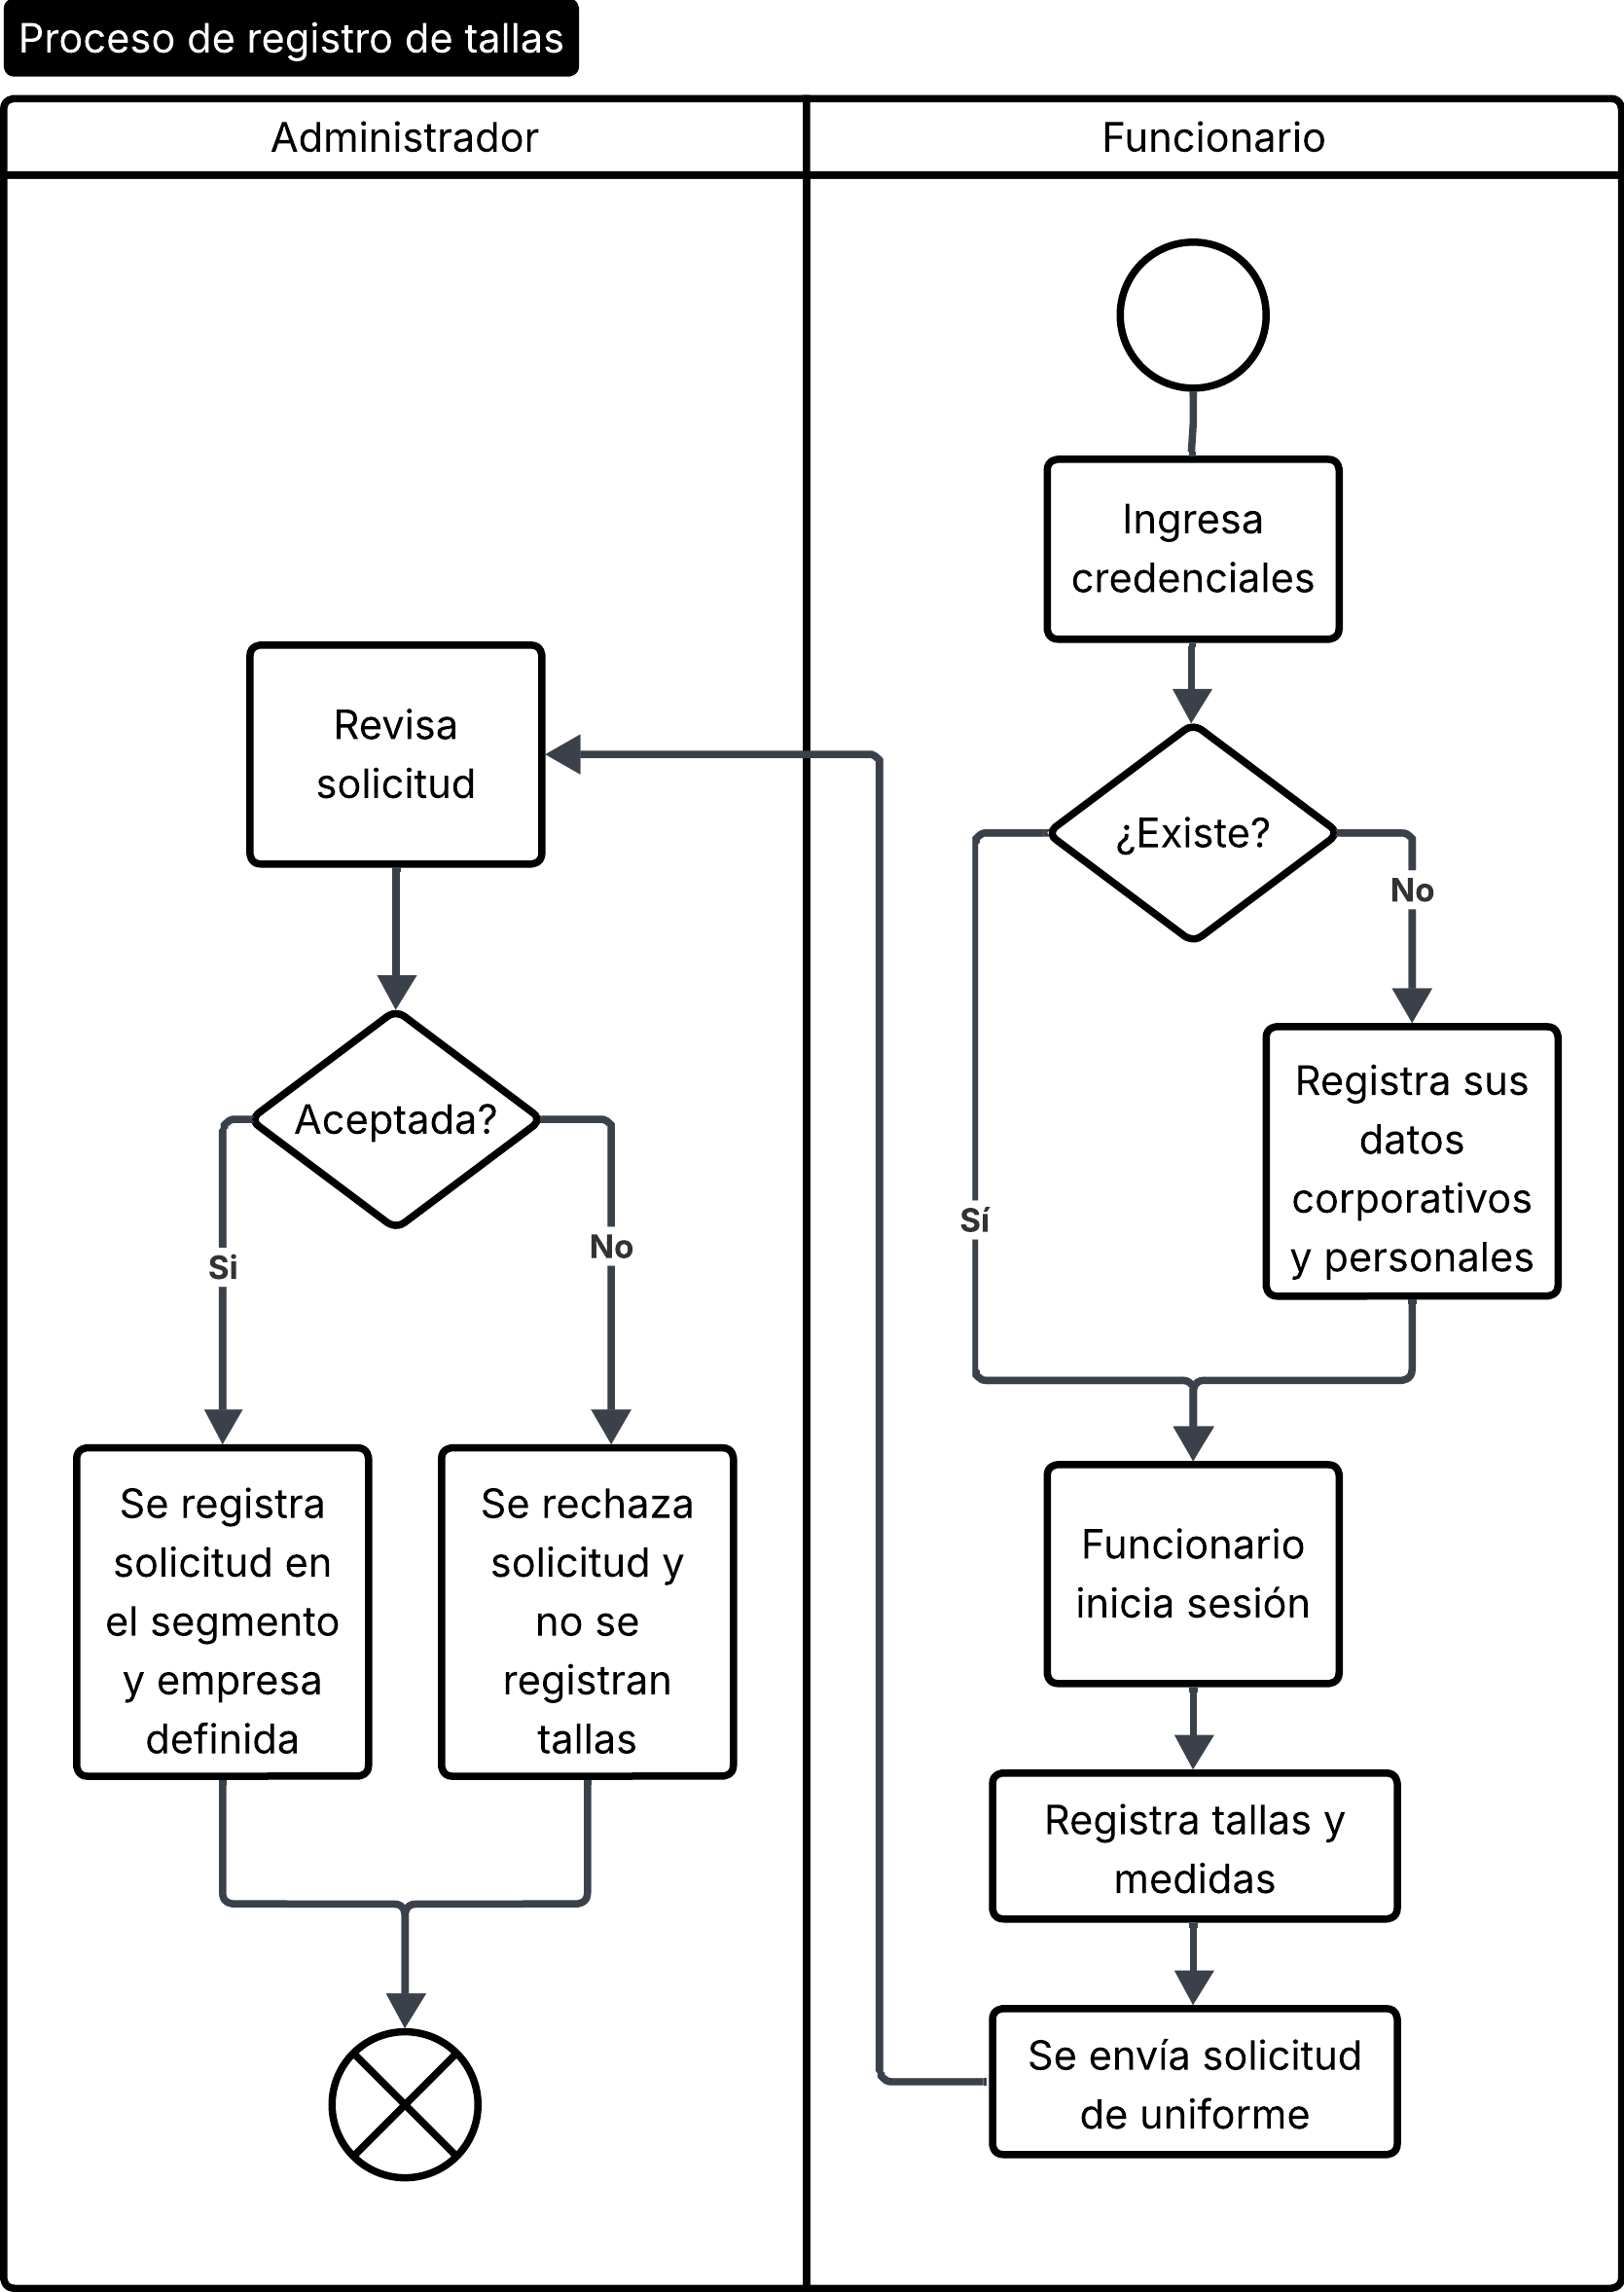
\includegraphics[height=0.9\textheight]{figuras/diagramas-actuales/diagrama-flujo-actual-registro-de-tallas.png}
    \caption{Diagrama de flujo del sistema actual sobre el proceso de registro de tallas}
    \label{fig:diagrama-flujo-actual-registro-de-tallas}
\end{figure}

\begin{figure}[htbp]
    \centering
    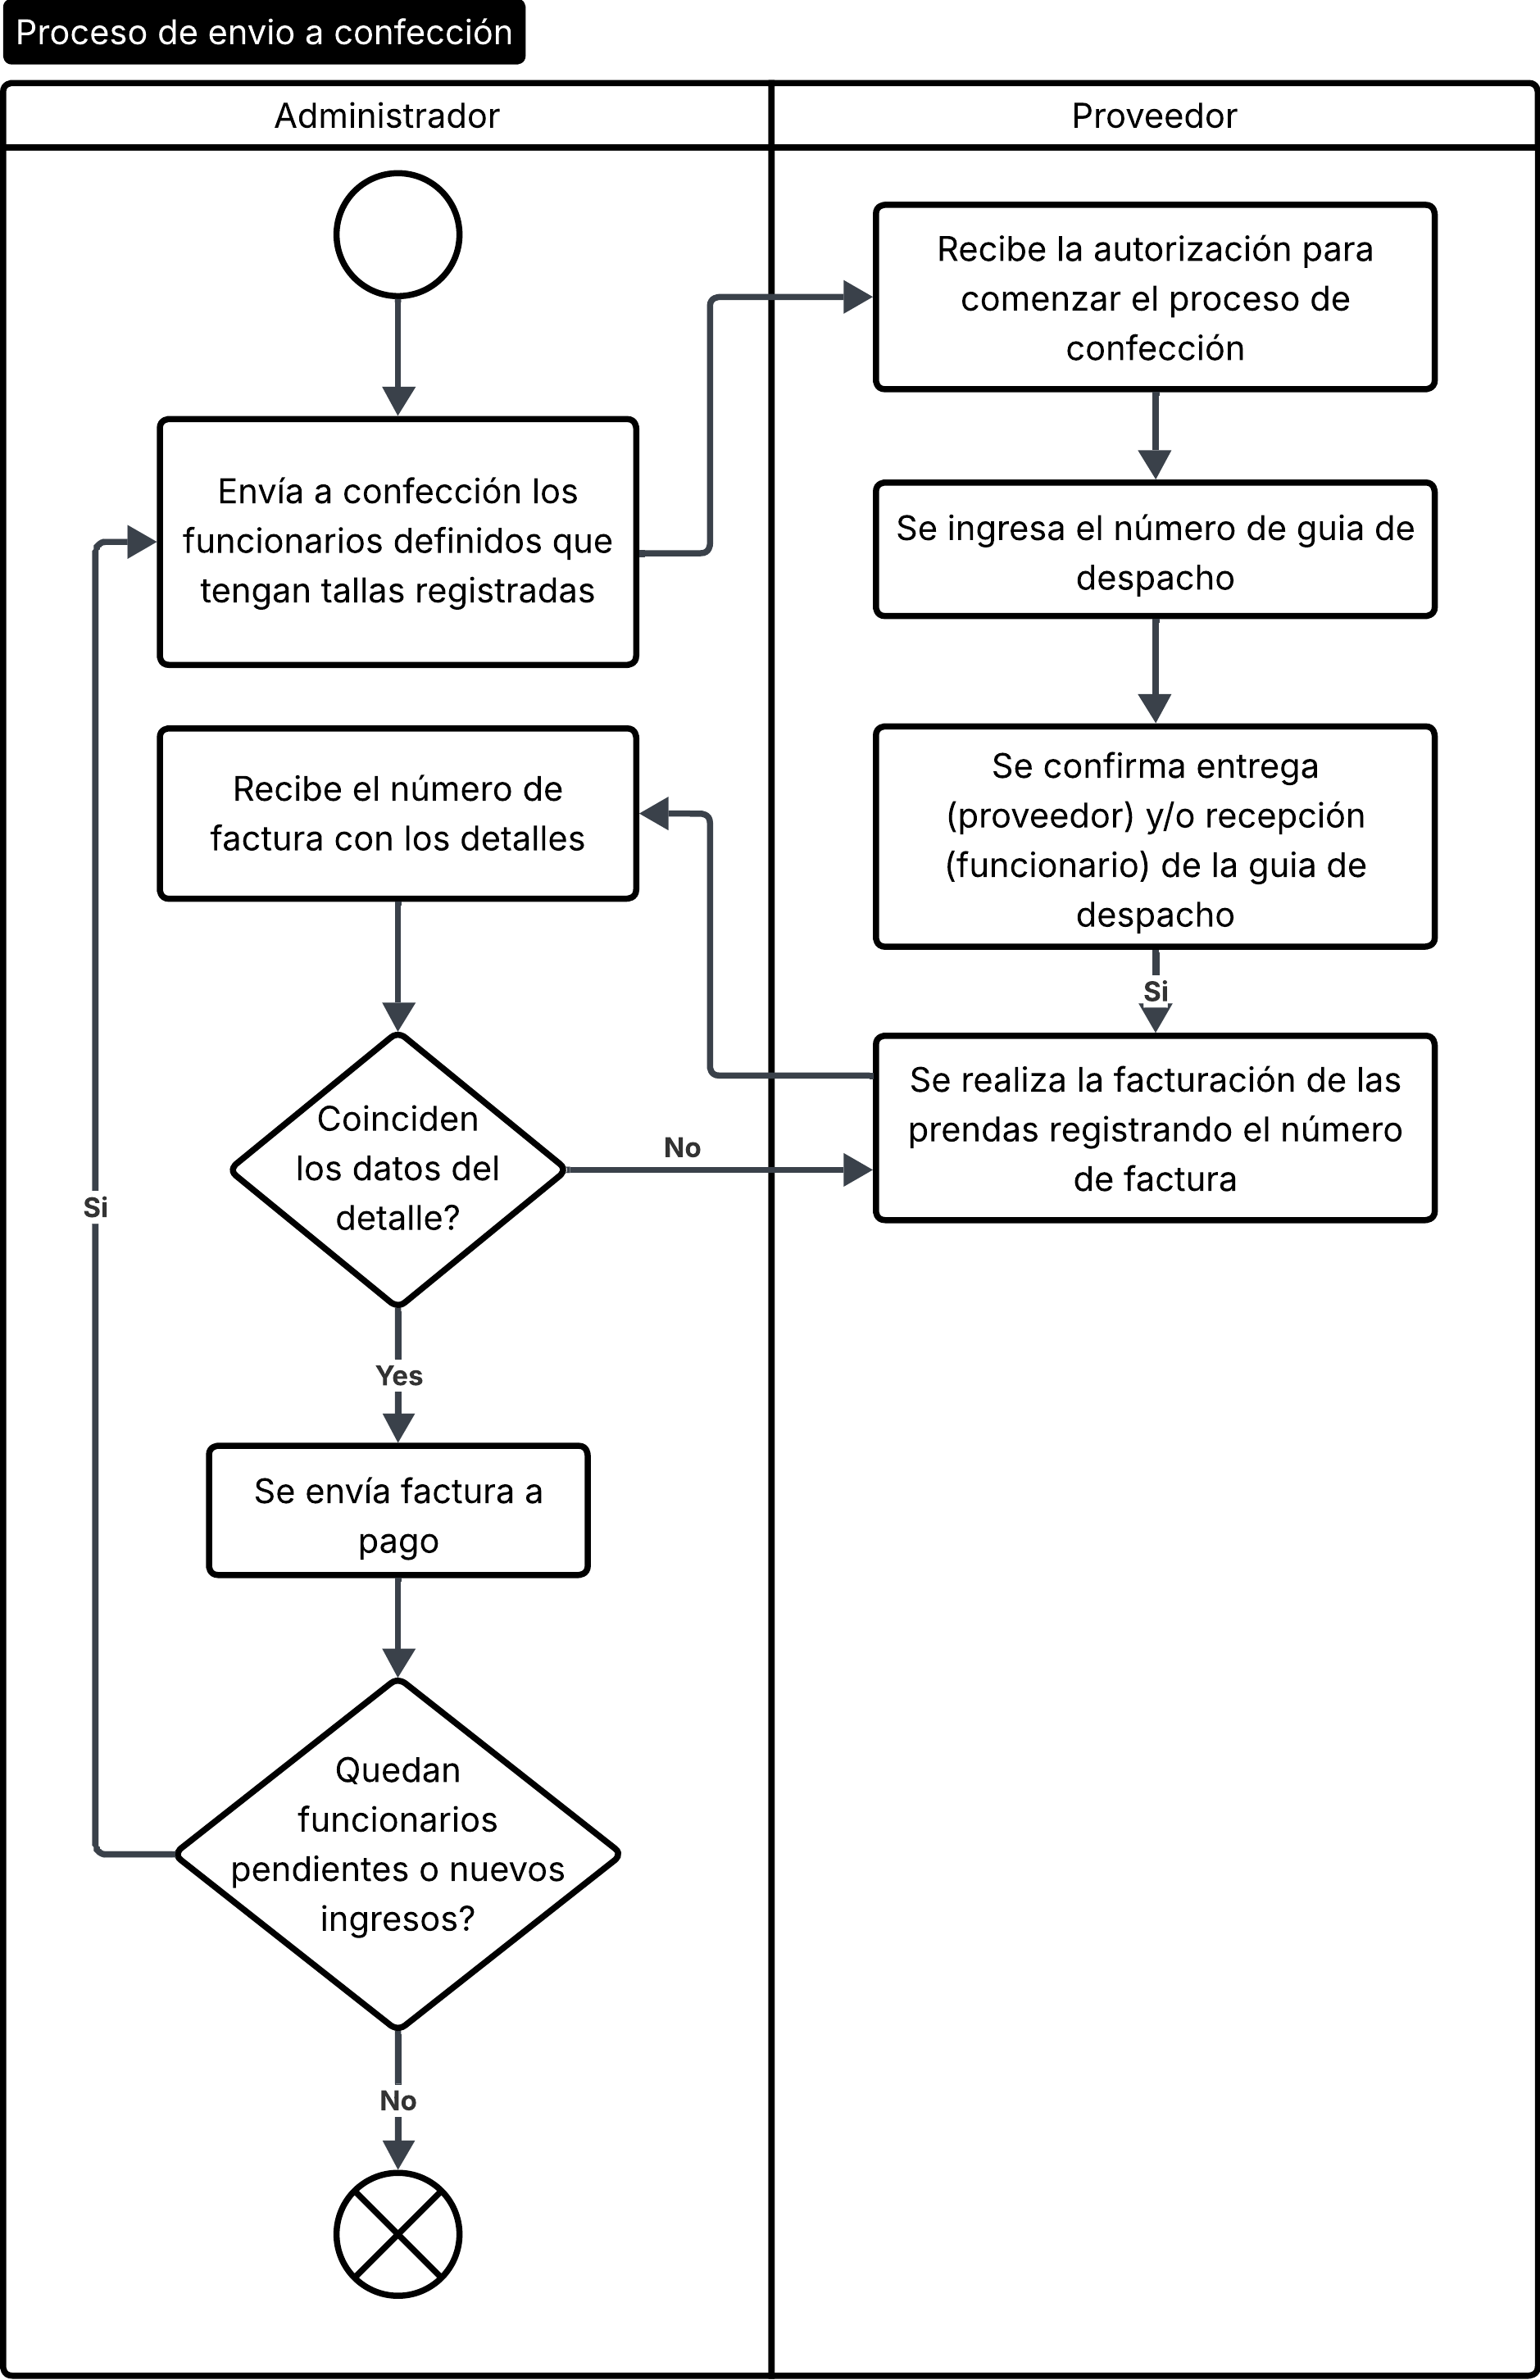
\includegraphics[height=0.9\textheight]{figuras/diagramas-actuales/diagrama-flujo-actual-envio-a-confeccion.png}
    \caption{Diagrama de flujo del sistema actual sobre el proceso de envío a confección}
    \label{fig:diagrama-flujo-actual-envio-a-confeccion}
\end{figure}

\begin{figure}[htbp]
    \centering
    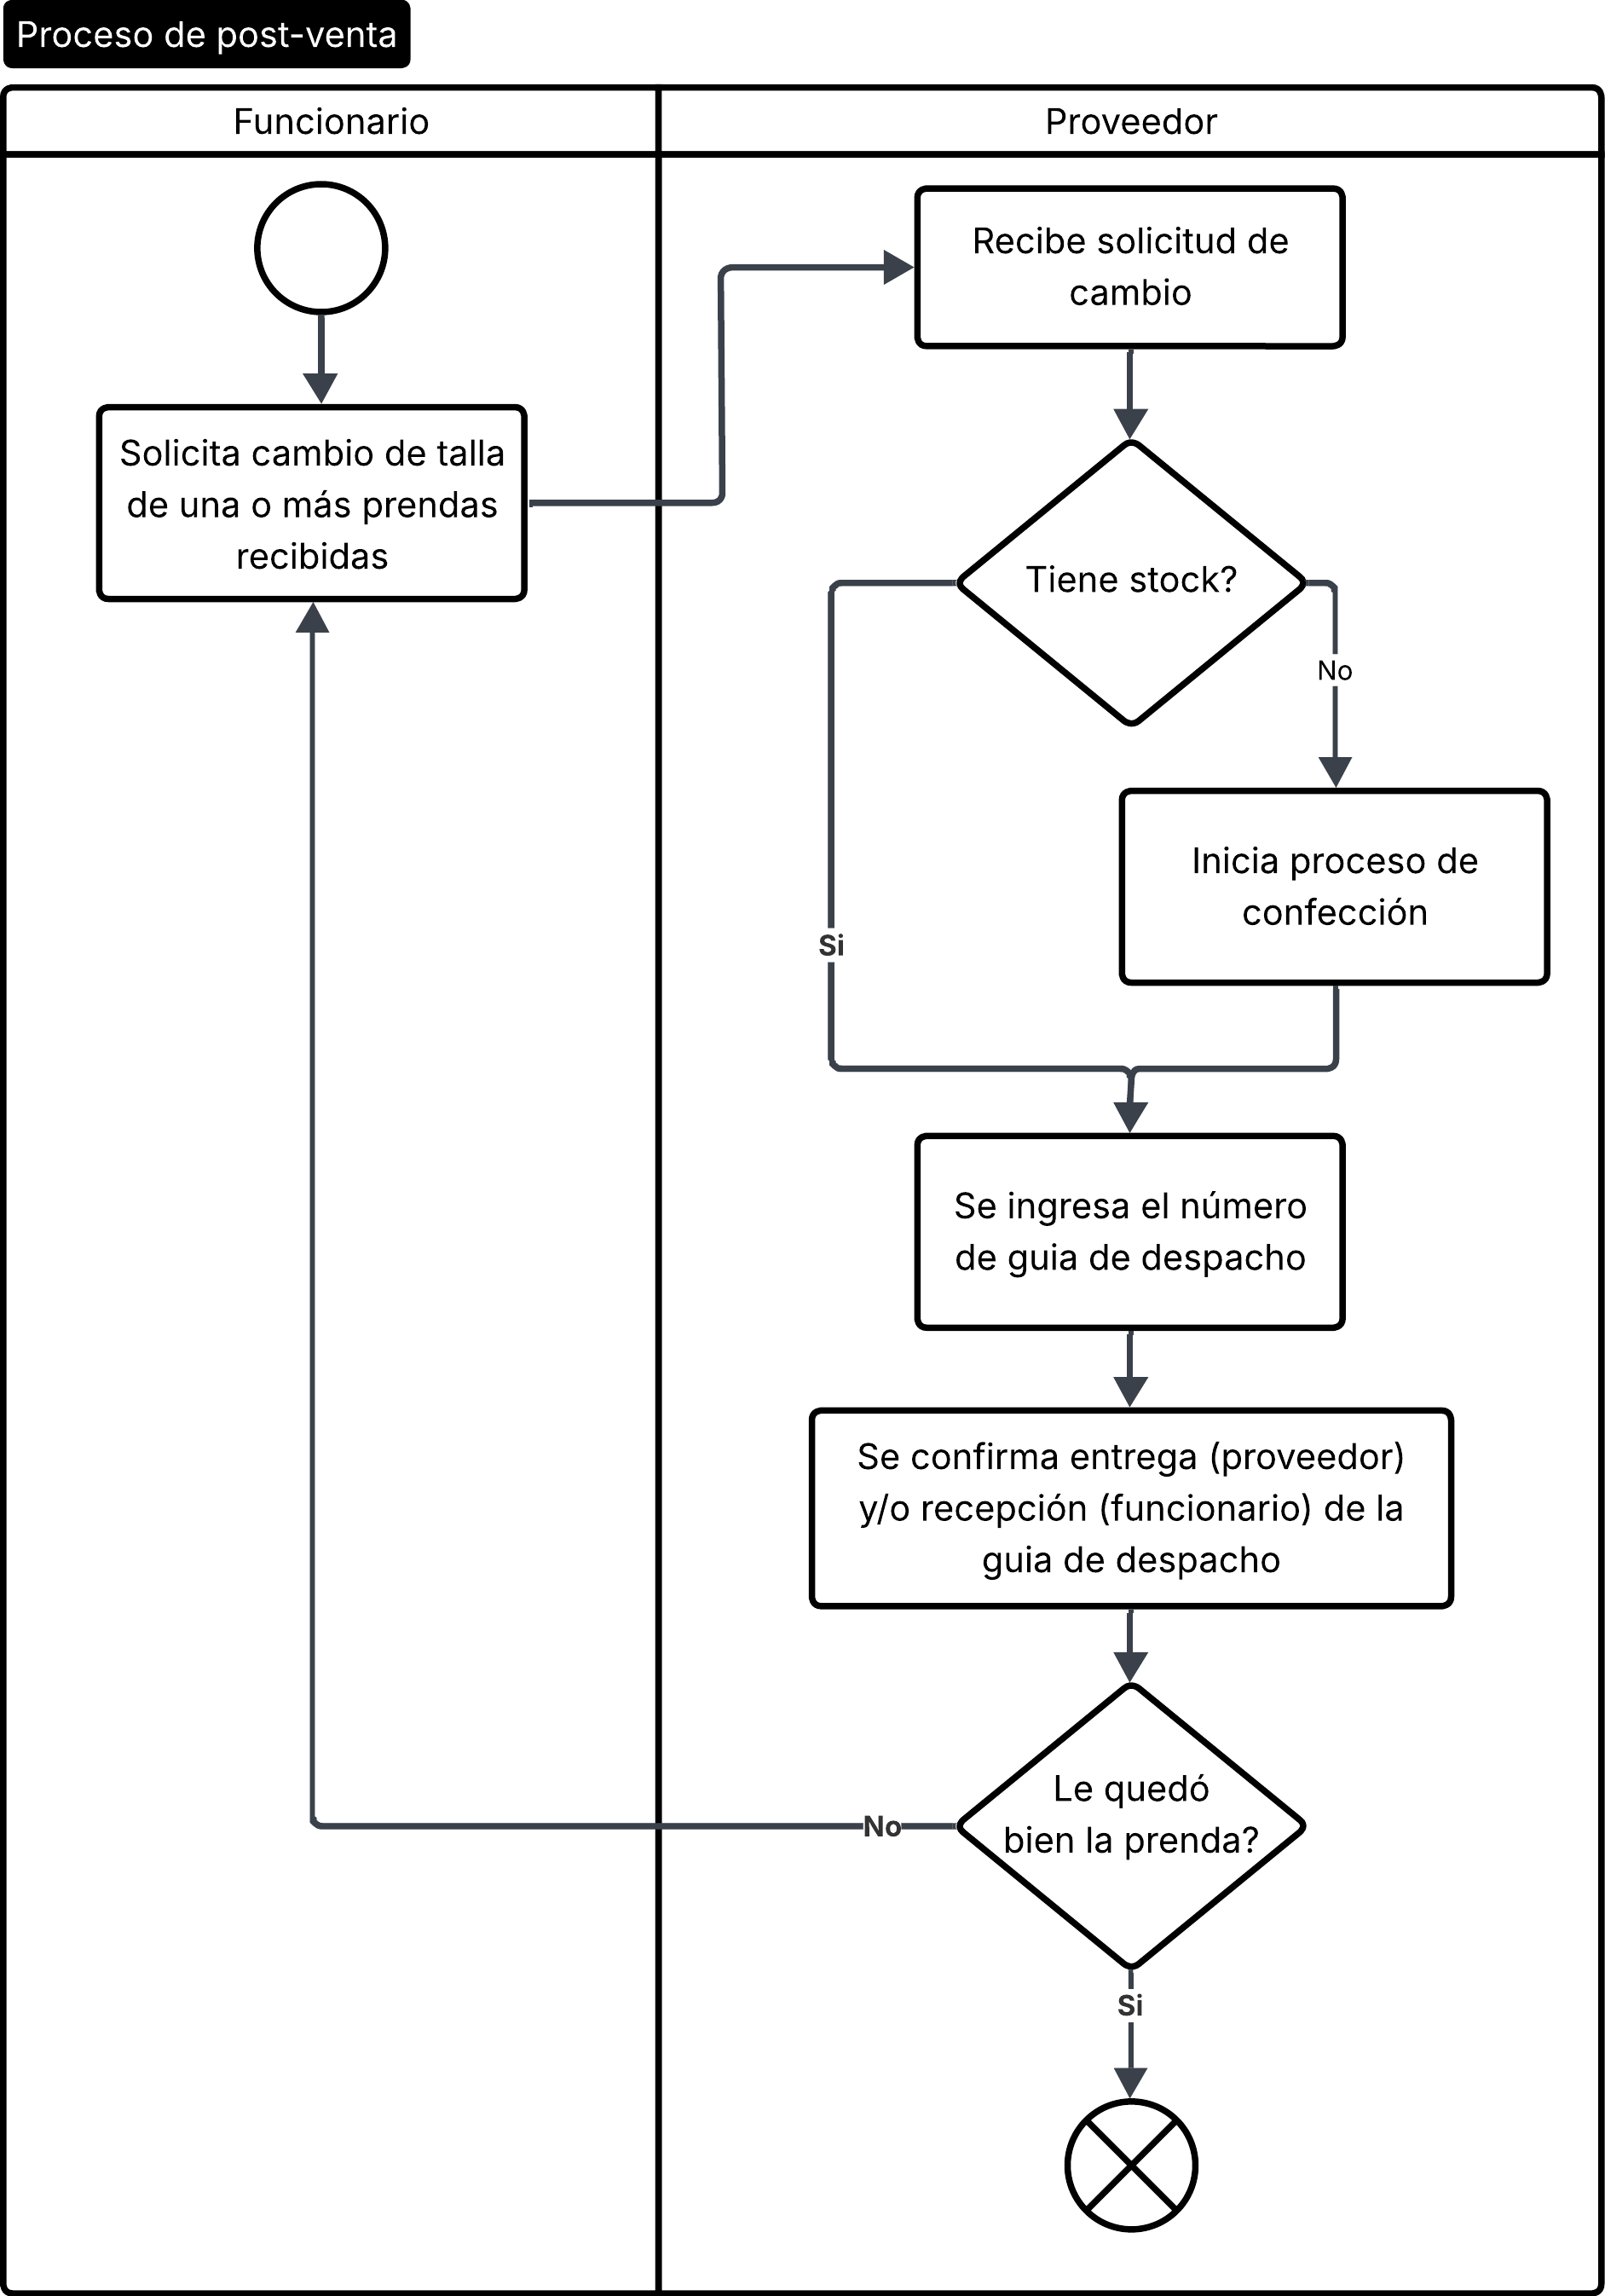
\includegraphics[height=0.9\textheight]{figuras/diagramas-actuales/diagrama-flujo-actual-post-venta.png}
    \caption{Diagrama de flujo del sistema actual sobre el proceso de post venta}
    \label{fig:diagrama-flujo-actual-post-venta}
\end{figure}

\subsection{Diagrama de Arquitectura}

En el diagrama de arquitectura actual (Figura \ref{fig:diagrama-arq-actual}) se aprecia la configuración monolítica del sistema, como este se encuentra alojado en BlueHosting que contienen ambos, el sistema y la base de datos. Con los actores principales conectándose a este mismo.

\begin{figure}[htbp]
    \centering
    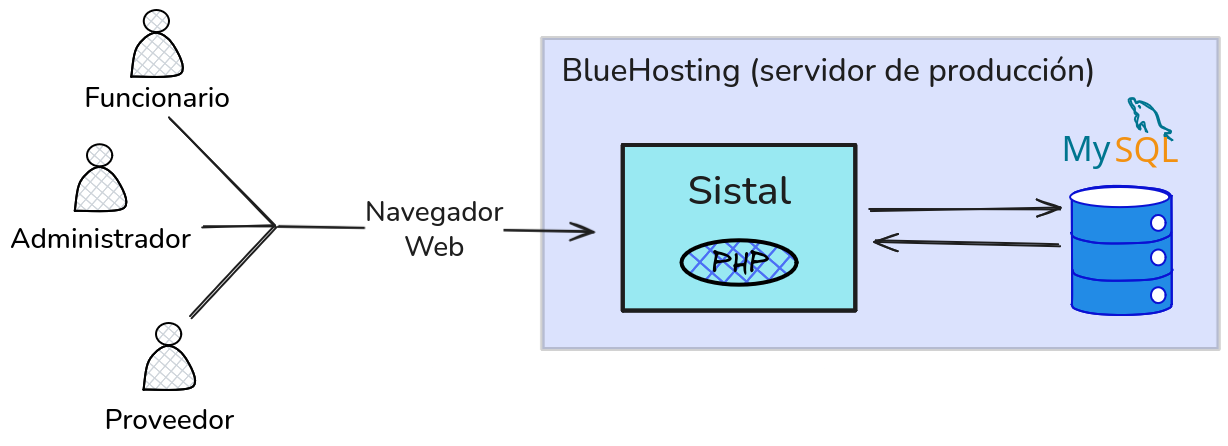
\includegraphics[width=\textwidth]{figuras/diagramas-actuales/diagrama-de-arquitectura}
    \caption{Diagrama de arquitectura del sistema actual}
    \label{fig:diagrama-arq-actual}
\end{figure}

\subsection{Diagrama de Despliegue}

En el diagrama de despliegue actual (Figura \ref{fig:diagrama-despliegue-actual})) se muestra el proceso manual de despliegue y actualización del sistema, en el que desde un entorno local, a través del protocolo \code{FTP/SFTP} se realiza una conexión al proveedor BlueHosting y se añaden/reemplazan el código del sistema.

\begin{figure}[htbp]
    \centering
    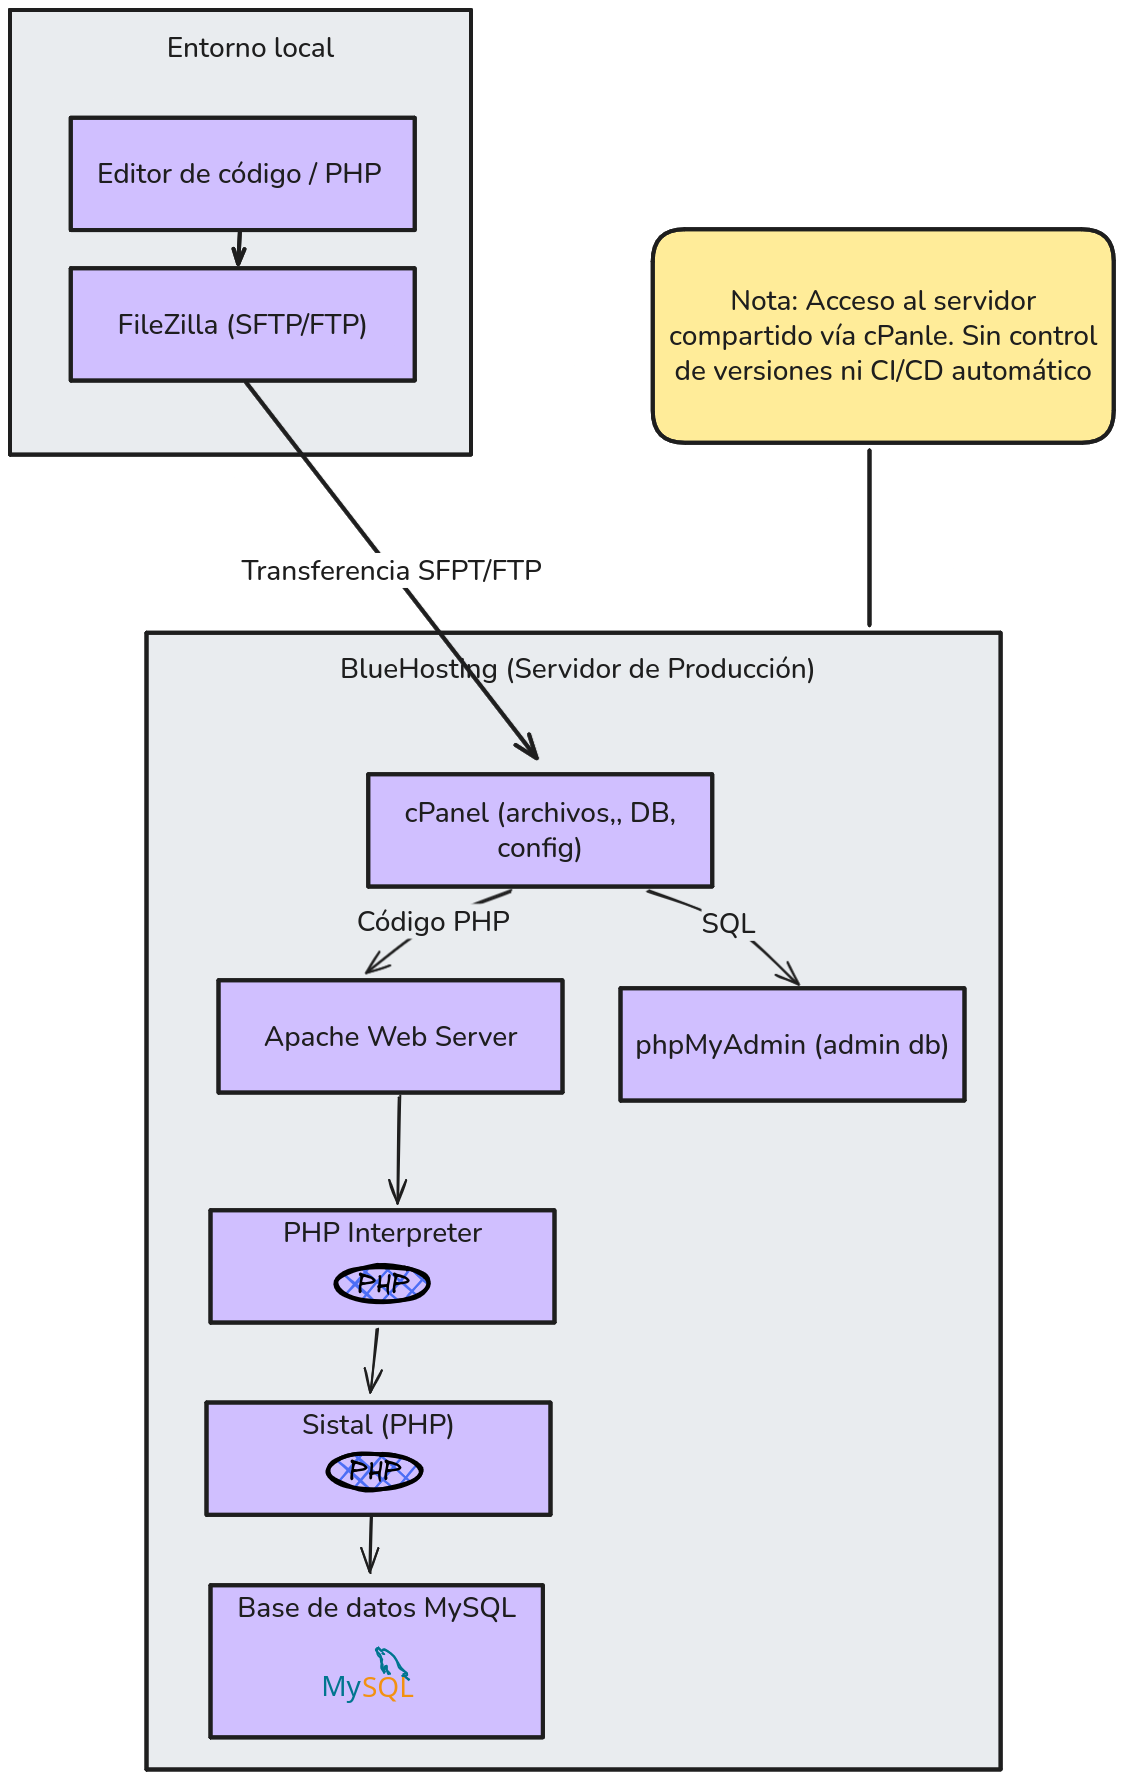
\includegraphics[height=0.9\textheight]{figuras/diagramas-actuales/diagrama-de-despliegue}
    \caption{Diagrama de despliegue del sistema actual}
    \label{fig:diagrama-despliegue-actual}
\end{figure}

